\documentclass[tikz,border=5pt]{standalone}
\usepackage[T1]{fontenc}
\usepackage{lmodern,amsmath,amssymb}
\usetikzlibrary{arrows.meta,calc,positioning,fit,backgrounds,shapes.geometric,matrix,decorations.pathreplacing,patterns}
\definecolor{ink}{gray}{0.08}
\definecolor{wash}{gray}{0.965}
\definecolor{soft}{gray}{0.45}
\tikzset{box/.style={draw=ink,line width=.65pt,fill=white,align=center,inner sep=4pt,outer sep=0pt,font=\small},flow/.style={draw=ink,line width=.65pt,-{Latex[length=1.8mm,width=1.3mm]},rounded corners=2pt},annotation/.style={font=\scriptsize,text=soft,align=center},groupbox/.style={draw=soft,dashed,line width=.45pt,fill=wash}}
\begin{document}
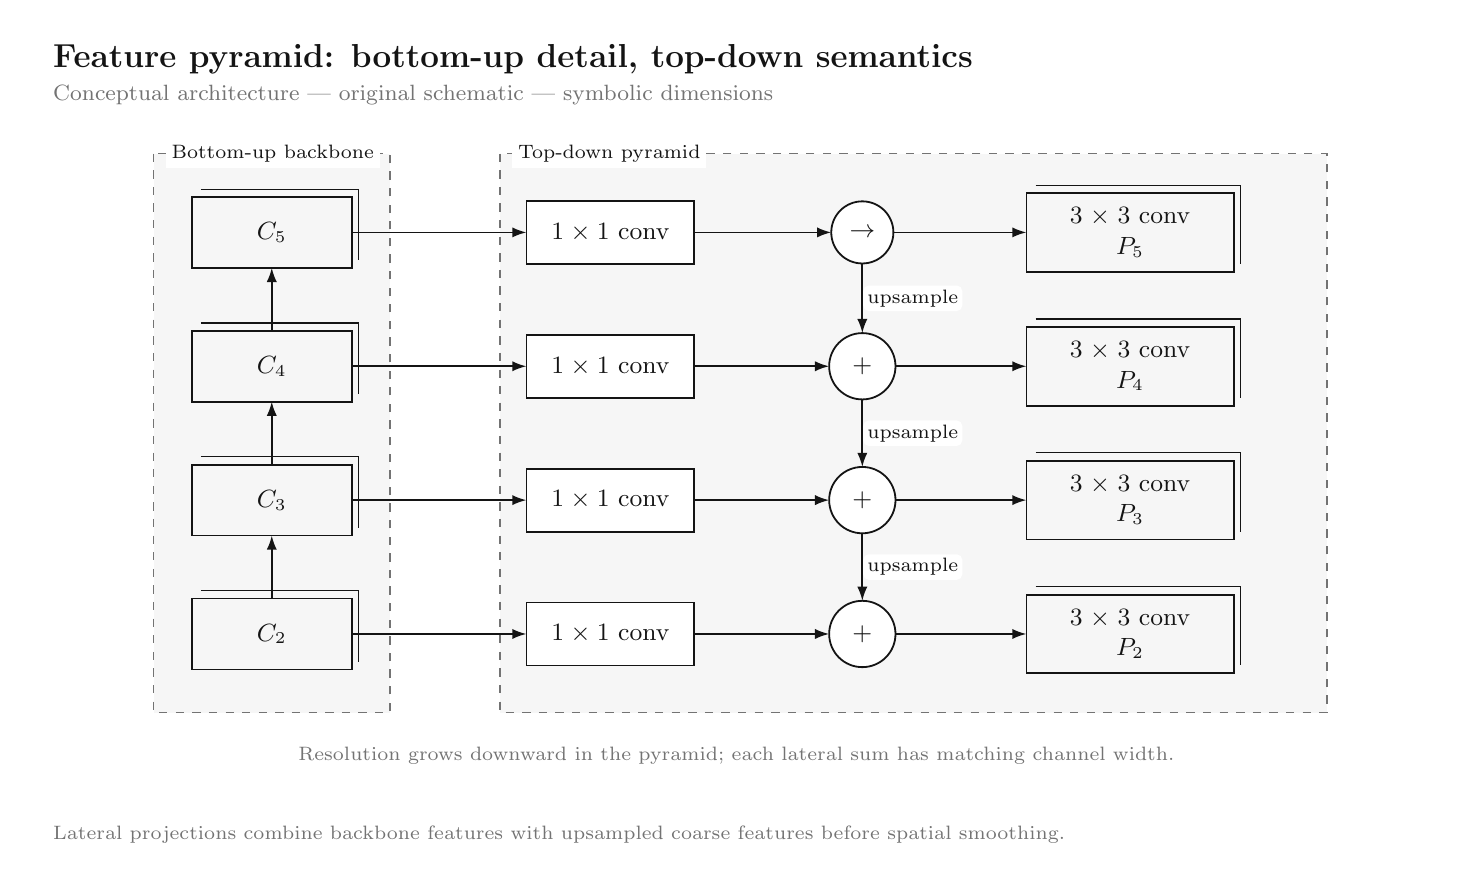
\begin{tikzpicture}[x=1cm,y=-1cm,font=\rmfamily,text=ink]

\path[use as bounding box] (0,0) rectangle (18,10.5);
\node[anchor=west,font=\large\bfseries] at (.2,.4) {Feature pyramid: bottom-up detail, top-down semantics};
\node[anchor=west,font=\footnotesize,text=soft] at (.2,.85) {Conceptual architecture | original schematic | symbolic dimensions};
\begin{pgfonlayer}{background}
\draw[groupbox] (1.6,1.6) rectangle (4.6,8.7);
\node[anchor=west,font=\scriptsize,fill=white,inner sep=2pt] at (1.75,1.6) {Bottom-up backbone};
\draw[groupbox] (6.0,1.6) rectangle (16.5,8.7);
\node[anchor=west,font=\scriptsize,fill=white,inner sep=2pt] at (6.15,1.6) {Top-down pyramid};
\end{pgfonlayer}
\node[box,fill=wash,minimum width=2.0cm,minimum height=0.9cm,text width=1.75cm] (c5) at (3.1,2.6) {$C_5$};
\draw[ink,line width=.4pt] (2.2,2.05) -- (4.199999999999999,2.05) -- (4.199999999999999,2.95);
\node[box,minimum width=2.1cm,minimum height=0.8cm,text width=1.85cm] (l5) at (7.4,2.6) {$1\times1$ conv};
\node[box,circle,minimum width=0.65cm,minimum height=0.65cm,text width=0.4cm] (m5) at (10.6,2.6) {$\rightarrow$};
\node[box,fill=wash,minimum width=2.6cm,minimum height=1.0cm,text width=2.35cm] (p5) at (14.0,2.6) {$3\times3$ conv\\$P_5$};
\draw[ink,line width=.4pt] (12.799999999999999,2.0) -- (15.4,2.0) -- (15.4,3.0);
\node[box,fill=wash,minimum width=2.0cm,minimum height=0.9cm,text width=1.75cm] (c4) at (3.1,4.3) {$C_4$};
\draw[ink,line width=.4pt] (2.2,3.7499999999999996) -- (4.199999999999999,3.7499999999999996) -- (4.199999999999999,4.65);
\node[box,minimum width=2.1cm,minimum height=0.8cm,text width=1.85cm] (l4) at (7.4,4.3) {$1\times1$ conv};
\node[box,circle,minimum width=0.65cm,minimum height=0.65cm,text width=0.4cm] (m4) at (10.6,4.3) {$+$};
\node[box,fill=wash,minimum width=2.6cm,minimum height=1.0cm,text width=2.35cm] (p4) at (14.0,4.3) {$3\times3$ conv\\$P_4$};
\draw[ink,line width=.4pt] (12.799999999999999,3.6999999999999997) -- (15.4,3.6999999999999997) -- (15.4,4.7);
\node[box,fill=wash,minimum width=2.0cm,minimum height=0.9cm,text width=1.75cm] (c3) at (3.1,6.0) {$C_3$};
\draw[ink,line width=.4pt] (2.2,5.45) -- (4.199999999999999,5.45) -- (4.199999999999999,6.3500000000000005);
\node[box,minimum width=2.1cm,minimum height=0.8cm,text width=1.85cm] (l3) at (7.4,6.0) {$1\times1$ conv};
\node[box,circle,minimum width=0.65cm,minimum height=0.65cm,text width=0.4cm] (m3) at (10.6,6.0) {$+$};
\node[box,fill=wash,minimum width=2.6cm,minimum height=1.0cm,text width=2.35cm] (p3) at (14.0,6.0) {$3\times3$ conv\\$P_3$};
\draw[ink,line width=.4pt] (12.799999999999999,5.4) -- (15.4,5.4) -- (15.4,6.4);
\node[box,fill=wash,minimum width=2.0cm,minimum height=0.9cm,text width=1.75cm] (c2) at (3.1,7.7) {$C_2$};
\draw[ink,line width=.4pt] (2.2,7.15) -- (4.199999999999999,7.15) -- (4.199999999999999,8.05);
\node[box,minimum width=2.1cm,minimum height=0.8cm,text width=1.85cm] (l2) at (7.4,7.7) {$1\times1$ conv};
\node[box,circle,minimum width=0.65cm,minimum height=0.65cm,text width=0.4cm] (m2) at (10.6,7.7) {$+$};
\node[box,fill=wash,minimum width=2.6cm,minimum height=1.0cm,text width=2.35cm] (p2) at (14.0,7.7) {$3\times3$ conv\\$P_2$};
\draw[ink,line width=.4pt] (12.799999999999999,7.1000000000000005) -- (15.4,7.1000000000000005) -- (15.4,8.1);
\begin{pgfonlayer}{background}
\draw[flow] (c5.east) -- (l5.west);
\draw[flow] (l5.east) -- (m5.west);
\draw[flow] (m5.east) -- (p5.west);
\draw[flow] (c4.east) -- (l4.west);
\draw[flow] (l4.east) -- (m4.west);
\draw[flow] (m4.east) -- (p4.west);
\draw[flow] (c3.east) -- (l3.west);
\draw[flow] (l3.east) -- (m3.west);
\draw[flow] (m3.east) -- (p3.west);
\draw[flow] (c2.east) -- (l2.west);
\draw[flow] (l2.east) -- (m2.west);
\draw[flow] (m2.east) -- (p2.west);
\draw[flow] (c4.north) -- (c5.south);
\draw[flow] (m5.south) -- (m4.north) node[midway,right,fill=white,inner sep=1.5pt,font=\scriptsize] {upsample};
\draw[flow] (c3.north) -- (c4.south);
\draw[flow] (m4.south) -- (m3.north) node[midway,right,fill=white,inner sep=1.5pt,font=\scriptsize] {upsample};
\draw[flow] (c2.north) -- (c3.south);
\draw[flow] (m3.south) -- (m2.north) node[midway,right,fill=white,inner sep=1.5pt,font=\scriptsize] {upsample};
\end{pgfonlayer}
\node[annotation,text width=14cm] at (9,9.25) {Resolution grows downward in the pyramid; each lateral sum has matching channel width.};
\node[anchor=west,align=left,font=\scriptsize,text=soft,text width=17.6cm] at (.2,10.25) {Lateral projections combine backbone features with upsampled coarse features before spatial smoothing.};
\end{tikzpicture}
\end{document}
